ee%%%%%%%%%%%%%%%%%%%%%%%%%%%%%%%%%%%%%%%%%%%%%%%%%%%%%%%%%%%%%%%%%%%%%%
%%  Copyright by Wenliang Du.                                       %%
%%  This work is licensed under the Creative Commons                %%
%%  Attribution-NonCommercial-ShareAlike 4.0 International License. %%
%%  To view a copy of this license, visit                           %%
%%  http://creativecommons.org/licenses/by-nc-sa/4.0/.              %%
%%%%%%%%%%%%%%%%%%%%%%%%%%%%%%%%%%%%%%%%%%%%%%%%%%%%%%%%%%%%%%%%%%%%%%

\newcommand{\commonfolder}{../../common-files}

\documentclass[11pt]{article}

\usepackage[most]{tcolorbox}
\usepackage{times}
\usepackage{epsf}
\usepackage{epsfig}
\usepackage{amsmath, alltt, amssymb, xspace}
\usepackage{wrapfig}
\usepackage{fancyhdr}
\usepackage{url}
\usepackage{verbatim}
\usepackage{fancyvrb}
\usepackage{adjustbox}
\usepackage{listings}
\usepackage{color}
\usepackage{subfigure}
\usepackage{cite}
\usepackage{sidecap}
\usepackage{pifont}
\usepackage{mdframed}
\usepackage{textcomp}
\usepackage{enumitem}
\usepackage{hyperref}


% Horizontal alignment
\topmargin      -0.50in  % distance to headers
\oddsidemargin  0.0in
\evensidemargin 0.0in
\textwidth      6.5in
\textheight     8.9in 

\newcommand{\todo}[1]{
\vspace{0.1in}
\fbox{\parbox{6in}{TODO: #1}}
\vspace{0.1in}
}


\newcommand{\unix}{{\tt Unix}\xspace}
\newcommand{\linux}{{\tt Linux}\xspace}
\newcommand{\minix}{{\tt Minix}\xspace}
\newcommand{\ubuntu}{{\tt Ubuntu}\xspace}
\newcommand{\setuid}{{\tt Set-UID}\xspace}
\newcommand{\openssl} {\texttt{openssl}}


\pagestyle{fancy}
\lhead{\bfseries SEED Labs}
\chead{}
\rhead{\small \thepage}
\lfoot{}
\cfoot{}
\rfoot{}


\definecolor{dkgreen}{rgb}{0,0.6,0}
\definecolor{gray}{rgb}{0.5,0.5,0.5}
\definecolor{mauve}{rgb}{0.58,0,0.82}
\definecolor{lightgray}{gray}{0.90}


\lstset{%
  frame=none,
  language=,
  backgroundcolor=\color{lightgray},
  aboveskip=3mm,
  belowskip=3mm,
  showstringspaces=false,
%  columns=flexible,
  basicstyle={\small\ttfamily},
  numbers=none,
  numberstyle=\tiny\color{gray},
  keywordstyle=\color{blue},
  commentstyle=\color{dkgreen},
  stringstyle=\color{mauve},
  breaklines=true,
  breakatwhitespace=true,
  tabsize=3,
  columns=fullflexible,
  keepspaces=true,
  escapeinside={(*@}{@*)}
}

\newcommand{\newnote}[1]{
\vspace{0.1in}
\noindent
\fbox{\parbox{1.0\textwidth}{\textbf{Note:} #1}}
%\vspace{0.1in}
}


%% Submission
\newcommand{\seedsubmission}{
Debe enviar un informe de laboratorio detallado, con capturas de pantalla, para describir lo que ha hecho y lo que ha observado.
También debe proporcionar una explicación a las observaciones que sean interesantes o sorprendentes.
Enumere también los fragmentos de código más importantes seguidos de una explicación. No recibirán créditos aquellos fragmentos de códigos que no sean explicados.}

%% Book
\newcommand{\seedbook}{\textit{Computer \& Internet Security: A Hands-on Approach}, 2nd
Edition, by Wenliang Du. Para más detalles \url{https://www.handsonsecurity.net}.\xspace}

%% Videos
\newcommand{\seedisvideo}{\textit{Internet Security: A Hands-on Approach},
by Wenliang Du. Para más detalles \url{https://www.handsonsecurity.net/video.html}.\xspace}

\newcommand{\seedcsvideo}{\textit{Computer Security: A Hands-on Approach},
by Wenliang Du. Para más detalles \url{https://www.handsonsecurity.net/video.html}.\xspace}

%% Lab Environment
\newcommand{\seedenvironment}{Este laboratorio ha sido testeado en nuestra imagen pre-compilada de una VM con Ubuntu 16.04, que puede ser descargada del sitio oficial de SEED.\xspace}

\newcommand{\seedenvironmentA}{Este laboratorio ha sido testeado en nuestra imagen pre-compilada de una VM con Ubuntu 16.04, que puede ser descargada del sitio oficial de SEED.\xspace}

\newcommand{\seedenvironmentB}{Este laboratorio ha sido testeado en nuestra imagen pre-compilada de una VM con Ubuntu 20.04, que puede ser descargada del sitio oficial de SEED .\xspace}

\newcommand{\seedenvironmentC}{Este laboratorio ha sido testeado en nuestra imagen pre-compilada de una VM con Ubuntu 20.04, que puede ser descargada del sitio oficial de SEED. Sin embargo, la mayoría de nuestros laboratorios pueden ser realizados en la nube para esto Ud. puede leer nuestra guía que explica como crear una VM de SEED en la nube.\xspace}

\newcommand{\seedenvironmentAB}{
Este laboratorio ha sido testeado en nuestras imagenes pre-compiladas de una VM con Ubuntu 16.04 y otra con Ubuntu 20.04, que pueden ser descargadas del sitio oficial de SEED.\xspace}

\newcommand{\nodependency}{Dado que utilizamos contenedores para configurar el entorno de laboratorio, este laboratorio no depende estrictamente de la VM de SEED. Puede hacer este laboratorio utilizando otras máquinas virtuales, máquinas físicas o máquinas virtuales en la nube.\xspace}

\newcommand{\adddns}{You do need to add the required IP address mapping to
the \texttt{/etc/hosts} file.\xspace}






\newcommand{\seedlabcopyright}[1]{
\vspace{0.1in}
\fbox{\parbox{6in}{\small Copyright \copyright\ {#1}\ \ by Wenliang Du.\\
      Este trabajo se encuentra bajo licencia Creative Commons.
       Attribution-NonCommercial-ShareAlike 4.0 International License.
       Si ud. remezcla, transforma y construye a partir de este material,
       Este aviso de derechos de autor debe dejarse intacto o reproducirse de una manera que sea razonable para el medio en el que se vuelve a publicar el trabajo.
       }}
\vspace{0.1in}
}






\newcommand{\dnsFigs}{./Figs}

\lhead{\bfseries SEED Labs -- Laboratorio de Ataque Remoto DNS - DNS cache poisoning}


\def \code#1 {\fbox{\scriptsize{\texttt{#1}}}}

\begin{document}

\begin{center}
{\LARGE Laboratorio del Ataque de Kaminsky}
\end{center}

\seedlabcopyright{2006 - 2020}


% *******************************************
% SECTION
% ******************************************* 
\section{Descripción del Laboratorio}

El objetivo de este laboratorio es que los estudiantes aprendan y experimenten con el ataque remoto al DNS, en particular DNS cache poisoning attack, también llamado el ataque de Kaminsky. 
DNS (Domain Name System o Sistema de nombre de Dominios) es la guía de teléfono de la Internet; se encarga de traducir los hostnames a direcciones IP (y visce versa). Esta traducción se hace a través de la resolución DNS, esta ocurre detrás de escena. Los ataques DNS manipulan este proceso de resolucion en varias maneras, con la intención de desviar a los usuarios a destinos alternativos, que a menudo son maliciosos. 
Este laboratorio se focaliza en una técnica particular de ataque al DNS, llamada {\em DNS Cache Poisoning attack}. 
En otro laboratorio SEED, hemos diseñado actividades para conducir el mismo ataque pero en un entorno de red loocal, es decir servidor DNS al cual tiene acceso el atacante y la víctima se encuentran en la misma red, donde es posible hacer sniffeo de paquetes.
En este laboratorio trataremos el ataque remoto al DNS donde no es posible hacer sniffing, por lo que el ataque se vuelve un poco más complejo y desafiante que el ataque local.
 
Este laboratorio cubre los siguientes tópicos:


\begin{itemize}[noitemsep]
\item DNS y su funcionamiento
\item Setup del servidor DNS
\item Ataque DNS cache poisoning
\item Spoofeando respuestas DNS
\item Spoofeo de Paquetes
\end{itemize}


\paragraph{Lecturas y Videos.}
Para una cobertura más detallada sobre el protocolo DNS y sus ataques puede consultar:

\begin{itemize}
\item Capítulo 18 del libro de SEED, \seedbook
\item Sección 7 del curso de SEED en Udemy, \seedisvideo
\end{itemize}


\paragraph{Entorno de Laboratorio.} \seedenvironmentC


%% Temporarily remove this part, to make the task a little bit simpler
%% during the transition phase (from VM to container)
\begin{comment}
\vspace{0.2in}
\noindent
\fbox{\parbox{\textwidth}{
\noindent
\textbf{Personalización.}
En la descripción de este laboratio usamos el dominio \texttt{attacker32.com} para referirnos al dominio que es controlado por el atacante. Cuando los estudiantes hagan este laboratorio, no se les permitirá usar este nombre; en lugar de esto deben de usar un nombre de dominio que incluya su apellido.
El objetivo de esto es diferenciar el trabajo de cada uno de los estudiantes. Dado que el nombre del dominio es visible solamente dentro del entorno del laboratorio y no por fuera de este, es posible usar este tipo de nombre de forma segura.
}}
\end{comment}




% *******************************************
% SECTION
% ******************************************* 
\section{Setup del Entorno de Laboratorio (Tarea 1)}
\label{sec:environment}

\begin{figure}[htb]
\centering
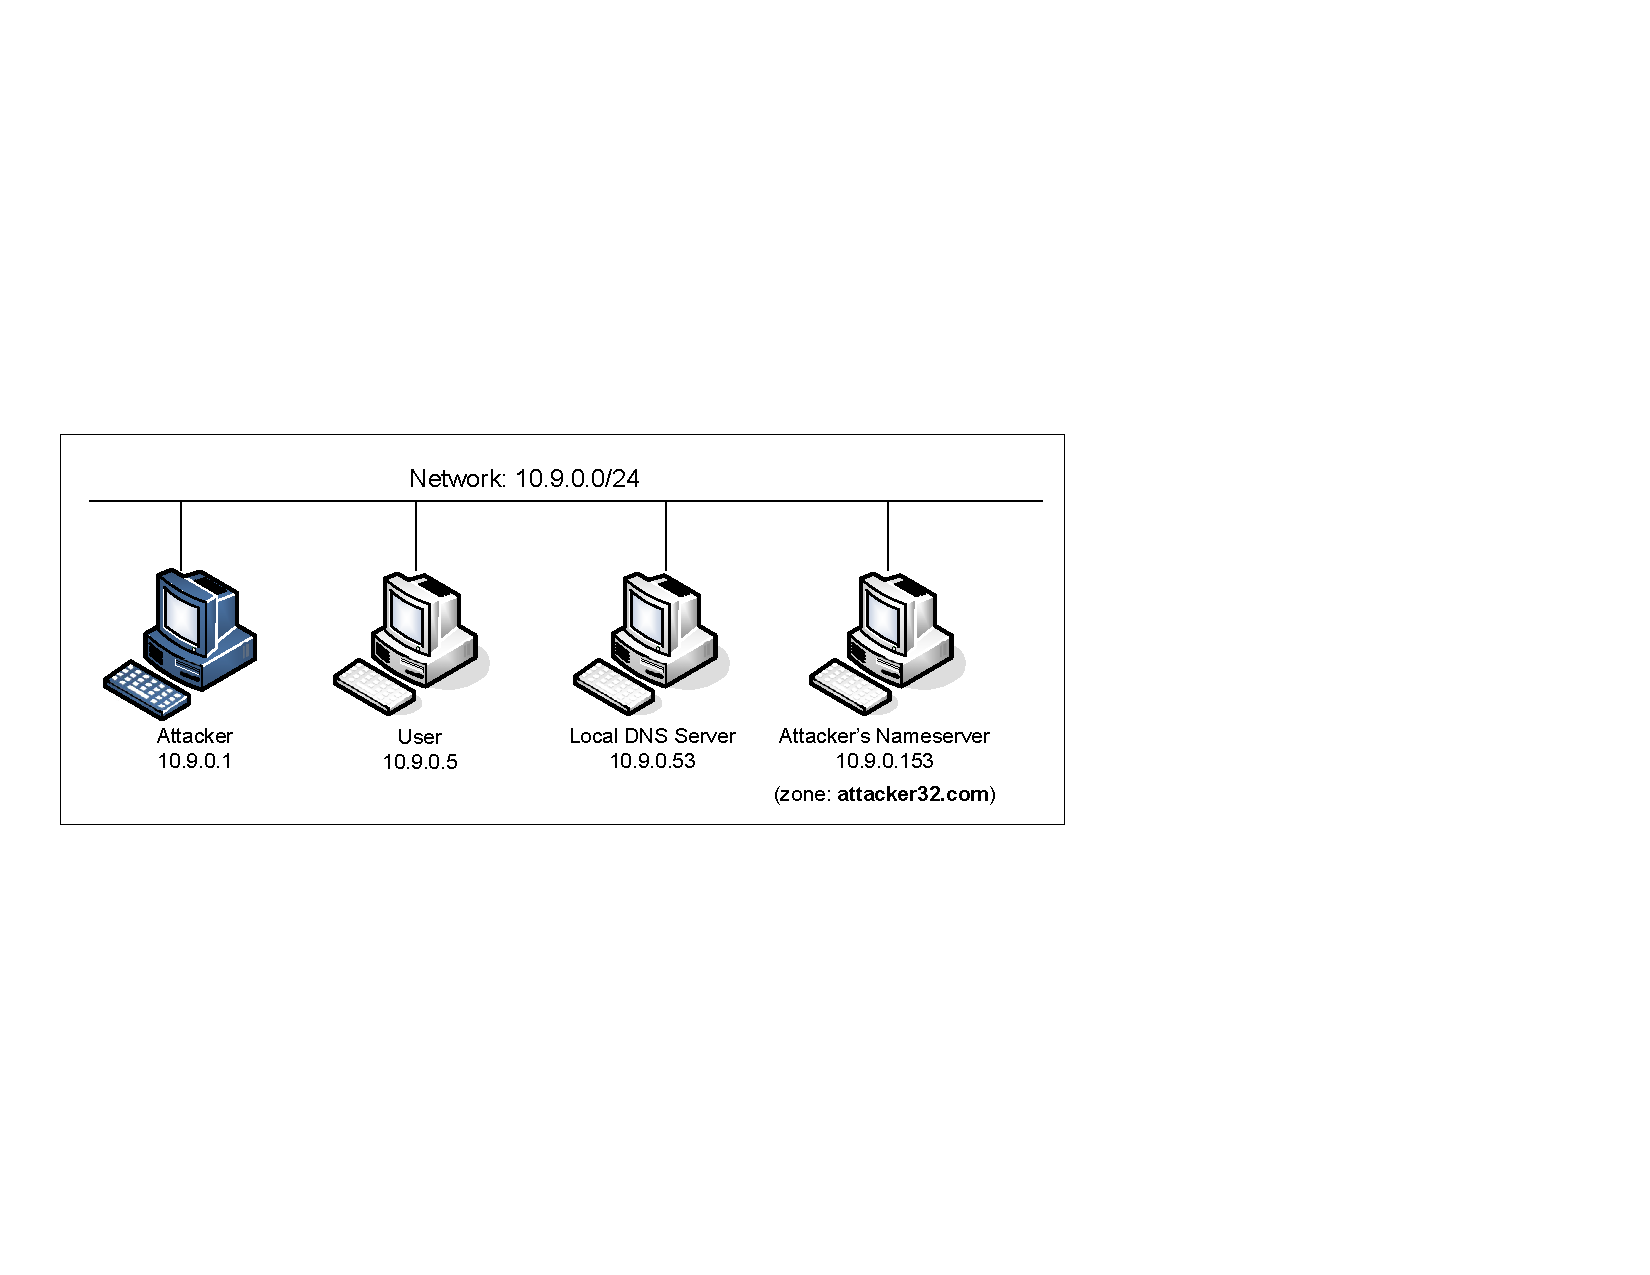
\includegraphics[width=0.85\textwidth]{\commonfolder/Figs/DNS.pdf}
\caption{Setup del Entorno}
\label{dns:fig:environment}
\end{figure}

El principal objetivo para un ataque de DNS cache poisoning es el servidor de DNS  local. Obviamente es ilegal atacar un servidor real, poor lo que necesitaremos crear y configurar nuestro propio servidor DNS para conducir los ataques en nuestros experimentos. El entorno de laboratorio necesita cuatro máquinas por separado:
una va a ser la máquina víctima, la segunda será el servidor de DNS local y las dos restantes serán las máquinas de los atacantes.
El setup del entorno del laboratorio se ilustra en la Figura \ref{dns:fig:environment}.


%\begin{lstlisting}[backgroundcolor=]
% +------------+   +------------+  +------------+  +---------------+
% | Attack VM  |   |  Container |  |  Container |  |  Container    |
% |            |   |   (user)   |  |  Local DNS |  |attacker32.com |
% |            |   |            |  |   Server   |  |  nameserver   |
% |  10.9.0.1  |   |  10.9.0.5  |  |  10.9.0.53 |  |  10.9.0.153   |
% +-----+------+   +------+-----+  +------+-----+  +------+--------+
%       |                 |               |               |
%       |                 |               |               |
%-------+-----------------+---------------+---------------+-------
%           Network  10.9.0.0/24
%
%\end{lstlisting}

Hemos puesto a todas las máquinas en la misma LAN con el objetivo de facilitar un poco todo.
Los estudiantes no pueden explotar este hecho en sus ataques; ellos deberían de considerar a la máquina del atacante como una máquina remota, es decir, el atacante no puede sniffear paquetes en la LAN.
Esto es diferente al ataque local del DNS.


% -------------------------------------------
% SUBSECTION
% -------------------------------------------
\subsection{Setup del Contenedor y sus Comandos}


%%%%%%%%%%%%%%%%%%%%%%%%%%%%%%%%%%%%%%%%%%%%
Para empezar a preparar el contenedor, deberá descargarse el archivo \texttt{Labsetup.zip} ubicado en el laboratorio correspondiente dentro del sitio web oficial y copiarlo dentro de la Máquina Virtual prevista por SEED. Una vez descargado deberá descomprimirlo y entrar dentro del directorio \texttt{Labsetup} donde encontrará el archivo \texttt{docker-compose.yml} que servirá para setear el entorno de laboratorio. Para una información más detallada sobre el archivo \texttt{Dockerfile} y otros archivos relacionados, puede encontrarla dentro del Manual de Usuario del laboratorio en uso, en el sitio web oficial de SEED.

Si esta es su primera experiencia haciendo el setup del laboratorio usando contenedores es recomendable que lea el manual anteriormente mencionado.

A continuación, se muestran los comandos más usados en Docker y Compose.
Debido a que estos comandos serán usados con mucha frecuencia, hemos creados un conjunto de alias para los mismos, ubicados en del archivo \texttt{.bashrc} dentro de la Máquina Virtual provista por SEED (Ubuntu 20.04)

\begin{lstlisting}
$ docker-compose build  # Build the container image
$ docker-compose up     # Start the container
$ docker-compose down   # Shut down the container

// Aliases for the Compose commands above
$ dcbuild       # Alias for: docker-compose build
$ dcup          # Alias for: docker-compose up
$ dcdown        # Alias for: docker-compose down
\end{lstlisting}


Dado que todos los contenedores estarán corriendo en un segundo plano. Necesitamos correr comandos para interactuar con los mismos, una de las operaciones fundamentales es obtener una shell en el contenedor. 
Para este propósito usaremos \texttt{"docker ps"} para encontrar el ID del contenedor deseado y ingresaremos \texttt{"docker exec"} para correr una shell en ese contenedor.
Hemos creado un alias para ello dentro del archivo \texttt{.bashrc}

\begin{lstlisting}
$ dockps        // Alias for: docker ps --format "{{.ID}}  {{.Names}}" 
$ docksh <id>   // Alias for: docker exec -it <id> /bin/bash

// The following example shows how to get a shell inside hostC
$ dockps
b1004832e275  hostA-10.9.0.5
0af4ea7a3e2e  hostB-10.9.0.6
9652715c8e0a  hostC-10.9.0.7

$ docksh 96
root@9652715c8e0a:/#  

// Note: If a docker command requires a container ID, you do not need to 
//       type the entire ID string. Typing the first few characters will 
//       be sufficient, as long as they are unique among all the containers. 
\end{lstlisting}

En caso de problemas configurando el entorno, por favor consulte la sección ``Common Problems'' en el manual ofrecido por SEED. 


%%%%%%%%%%%%%%%%%%%%%%%%%%%%%%%%%%%%%%%%%%%%



% -------------------------------------------
% SUBSECTION
% -------------------------------------------
\subsection{Sobre el Contenedor del Atacante}

Para este laboratorio podemos usar tanto una Máquina Virtual como un contenedor como máquina de ataque. Si observa el archivo Docker Compose, verá que el contenedor de ataque está configurado de forma diferente al resto de los contenedores.


\begin{itemize}
\item \textit{Directorio Compartido.} Cuando usemos el contenedor del atacante para realizar los ataques, necesitamos poner el código de ataque dentro del contenedor.
%%%%%%%%%%%%%%%%%%%%%%%%%%%%%%%%%%%%%%%%%%%%%%%
Code editing is more convenient inside the VM than in containers, 
because we can use our favorite editors.
In order for the VM and container to share files, 
we have created a shared folder between the VM and the container
using the Docker \texttt{volumes}.
If you look at the Docker Compose file, you will find out that
we have added the following entry to some of the containers.
It indicates mounting the \texttt{./volumes} folder on the host
machine (i.e., the VM) to the \texttt{/volumes} folder inside the container.
We will write our code in the \texttt{./volumes} folder (on the VM), so they
can be used inside the containers.

\begin{lstlisting}
volumes:
       - ./volumes:/volumes
\end{lstlisting}


%%%%%%%%%%%%%%%%%%%%%%%%%%%%%%%%%%%%%%%%%%%%%%%


\item \textit{Host mode.}
%%%%%%%%%%%%%%%%%%%%%%%%%%%%%%%%%%%%%%%%%%%%%%%
In this lab, the attacker needs to be able to sniff packets,
but running sniffer programs inside a container has problems, because
a container is effectively attached to a virtual switch, 
so it can only see its own traffic, and it is never going to see 
the packets among other containers. To solve this problem,
we use the \texttt{host} mode for the attacker container. This
allows the attacker container to see all the traffics. The following
entry used on the attacker container:

\begin{lstlisting}
network_mode: host
\end{lstlisting}

When a container is in the \texttt{host} mode,  it sees
all the host's network interfaces, and it even has the same
IP addresses as the host. Basically, it is put in the
same network namespace as the host VM. However, the container
is still a separate machine, because its other namespaces are
still different from the host.


%%%%%%%%%%%%%%%%%%%%%%%%%%%%%%%%%%%%%%%%%%%%%%%
\end{itemize}





% -------------------------------------------
% SUBSECTION
% -------------------------------------------
%%%%%%%%%%%%%%%%%%%%%%%%%%%%%%%%%%%%%%%%%%%%
%%%%%%%%%%%%%%%%%%%%%%%%%%%%%%%%%%%%%%%%%%%%%%%%%%%%%%%%%%%%%%%%%%%%%%
%%  Copyright by Wenliang Du.                                       %%
%%  This work is licensed under the Creative Commons                %%
%%  Attribution-NonCommercial-ShareAlike 4.0 International License. %%
%%  To view a copy of this license, visit                           %%
%%  http://creativecommons.org/licenses/by-nc-sa/4.0/.              %%
%%%%%%%%%%%%%%%%%%%%%%%%%%%%%%%%%%%%%%%%%%%%%%%%%%%%%%%%%%%%%%%%%%%%%%


% -------------------------------------------
% SUBSECTION
% ------------------------------------------- 
\subsection{Resumen de la Configuración del DNS} 

Todos los contenedores han sido configurados para este laboratorio.
Por lo que haremos un resumen de ellos, de esta manera los estudiantes estarán al tanto de estas configuraciones. Para explicaciones más detalladas sobre las configuraciones puede consultar el manual.



\paragraph{Servidor de DNS local.} 
Como servidor de DNS local usaremos el software BIND 9.
BIND 9 carga su configuración de un archivo llamado \path{/etc/bind/named.conf}. Este es el principal archivo de configuración y usualmente contiene varias entradas de \texttt{"include"}, por medio de este include puede cargar las configuraciones de diferentes archivos. Uno de los archivos usado por ese include es llamado \path{/etc/bind/named.conf.options}. Es en este archivo donde se establece la configuración actual.


\begin{itemize}
\item \textit{Simplificación.}
Los servidores DNS hoy en día randomizan el número de puerto de origen en sus consultas DNS; esto hace que los ataques sean mucho más difíciles. Desafortunadamente, muchos servidores DNS siguen usando número de puertos de origen predecibles. Para simplificar este laboratorio, hemos fijado el número de puerto de origen a {\tt 33333} dentro del archivo de configuración.

\item \textit{Desactivando DNSSEC.} 
DNSSEC fue introducido como mecanismo de protección en contra de ataques de spoofing en los servidores DNS. Para mostrar como funciona este ataque, hemos desactivado esta protección en el archivo de configuración.

\item \textit{DNS caché.}
Durante el ataque, necesitaremos inspeccionar la caché DNS en el servidor de DNS local. Los siguientes dos comando sirven para este propósito.
El primer comando hace un dump del contenido de la caché en el archivo \path{/var/cache/bind/dump.db}, y el segundo comando limpia la caché.

\begin{lstlisting}
# rndc dumpdb -cache    // Dump the cache to the specified file
# rndc flush            // Flush the DNS cache
\end{lstlisting}

\item \textit{Forwardeo de la zona \texttt{attacker32.com}.}
Una zona de forwardeo es agregada en el servidor de DNS local, por lo que si alguien quiere consultar el dominio \texttt{attacker32.com}, la consulta será forwardeada al nameserver de este dominio, que será hosteado en el contenedor del atacante. La entrada para esta zona se ubcica dentro del archivo \texttt{named.conf}.

\begin{lstlisting}
zone "attacker32.com" {
    type forward;
    forwarders { 
        10.9.0.153; 
    };
};
\end{lstlisting}
\end{itemize}



\paragraph{Máquina del Usuario.}
El contenedor del usuario cuya dirección IP es {\tt 10.9.0.5} está configurada para usar la dirección IP {\tt 10.9.0.53} como su servidor DNS local.
Esto se logra cambiando la configuración del archivo de resolución de la máquina del usuario (\texttt{/etc/resolv.conf}), se agrega el servidor \texttt{10.9.0.53}  como \texttt{nameserver} en la primera línea del archivo, de esta forma la máquina entenderá que este será el servidor DNS primario usado por defecto.


\paragraph{Nameserver del Atacante.}
Dentro de la máquina del atacante, se hostean dos zonas. La primera es la zona legítima del atacante \texttt{attacker32.com}, y la segunda es la zona falsa del dominio \texttt{example.com}. Las zonas son configuradas en el archivo \path{/etc/bind/named.conf}:

\begin{lstlisting}
zone "attacker32.com" {
        type master;
        file "/etc/bind/attacker32.com.zone";
};

zone "example.com" {
        type master;
        file "/etc/bind/example.com.zone";
};
\end{lstlisting}


%%%%%%%%%%%%%%%%%%%%%%%%%%%%%%%%%%%%%%%%%%%%%%%%%%%%%%%%%%%%%%%%%%%%%%
%%  Copyright by Wenliang Du.                                       %%
%%  This work is licensed under the Creative Commons                %%
%%  Attribution-NonCommercial-ShareAlike 4.0 International License. %%
%%  To view a copy of this license, visit                           %%
%%  http://creativecommons.org/licenses/by-nc-sa/4.0/.              %%
%%%%%%%%%%%%%%%%%%%%%%%%%%%%%%%%%%%%%%%%%%%%%%%%%%%%%%%%%%%%%%%%%%%%%%


% -------------------------------------------
% SUBSECTION
% ------------------------------------------- 
\subsection{Testing the DNS Setup}

From the User container, we will run a series of commands to ensure 
that our lab setup is correct. In your lab report, please document
your testing results. 


\paragraph{Get the IP address of \texttt{ns.attacker32.com}.}
When we run the following \texttt{dig} command, 
the local DNS server will forward the request to the Attacker nameserver 
due to the \texttt{forward} zone entry added to the local DNS server's
configuration file. Therefore, the answer should come from
the zone file (\texttt{attacker32.com.zone}) that we set up on the Attacker nameserver.
If this is not what you get, your setup has issues. Please describe your
observation in your lab report. 

\begin{lstlisting}
$ dig ns.attacker32.com
\end{lstlisting}



\paragraph{Get the IP address of \texttt{www.example.com}.} 
Two nameservers are now hosting the \texttt{example.com} 
domain, one is the domain's official nameserver, and the other 
is the Attacker container. We will query these two nameservers and see what 
response we will get. 
Please run the following two commands (from the User machine), 
and describe your observation. 


\begin{lstlisting}
// Send the query to our local DNS server, which will send the query
// to example.com's official nameserver. 
$ dig www.example.com

// Send the query directly to ns.attacker32.com 
$ dig @ns.attacker32.com www.example.com
\end{lstlisting}
 


Obviously, nobody is going to ask \texttt{ns.attacker32.com} for 
the IP address of \texttt{www.example.com}; they will always ask
the \texttt{example.com} domain's official nameserver for 
answers. The objective of the DNS cache poisoning attack
is to get the victims to ask 
\texttt{ns.attacker32.com} for the IP address of 
\texttt{www.example.com}. Namely, if our attack is successful, 
if we just run the first \texttt{dig} command, the one
without the \texttt{@} option, we should get the 
fake result from the attacker, instead of getting 
the authentic one from the domain's legitimate nameserver.



%%%%%%%%%%%%%%%%%%%%%%%%%%%%%%%%%%%%%%%%%%%%



% *******************************************
% SECTION
% ******************************************* 
\section{Las tareas de ataque}

El principal objetivo de los ataques DNS sobre un usuario es poder redireccionar al usuario hacia una máquina $B$ cuando el usuario intente acceder a una máquina $A$ usando el hostname de $A$. Por ejemplo, cuando un usuario trata de acceder al online banking, los atacantes pueden redireccionarlo a un sitio web malicioso que luce casi igual al sitio oficial del banco, en consecuencia el usuario puede ser engañado y así los atacantes pueden obtener sus credenciales bancarias.

En esta tarea, vamos a usar el nombre de dominio {\tt www.example.com} como nuestro objetivo para hacer el ataque. Cabe señalar que el dominio {\tt www.example.com} está reservado solamente para el uso experimental dentro del contexto de este laboratorio y no para el mundo real. La dirección IP real de {\tt www.example.com} es {\tt 93.184.216.34} y su nameserver es controlado por la Internet Corporation for Assigned Names and Numbers (ICANN).
Cuando el usuario ejecuta el comando {\tt dig} sobre este dominio o usa el navegador para visitarlo, la máquina del usuario envia una consulta DNS a su servidor de DNS local que consultará la dirección IP usando el nameserver de {\tt example.com}.

La meta del ataque es ejecutar un ataque de DNS cache poisoning attack en el servidor de DNS local, de tal forma que cuando el usuario ejecute el comando {\tt dig} para obtener la dirección IP de {\tt www.example.com}, el servidor de DNS local terminará consultando el nameserver del atacante {\tt ns.attacker32.com} y así obtendrá la dirección IP definida por atacante. Como resultado final el usuario será dirigido al sitio web del atacante en lugar del sitio original {\tt www.example.com}.



\begin{figure}[htb]
\centering
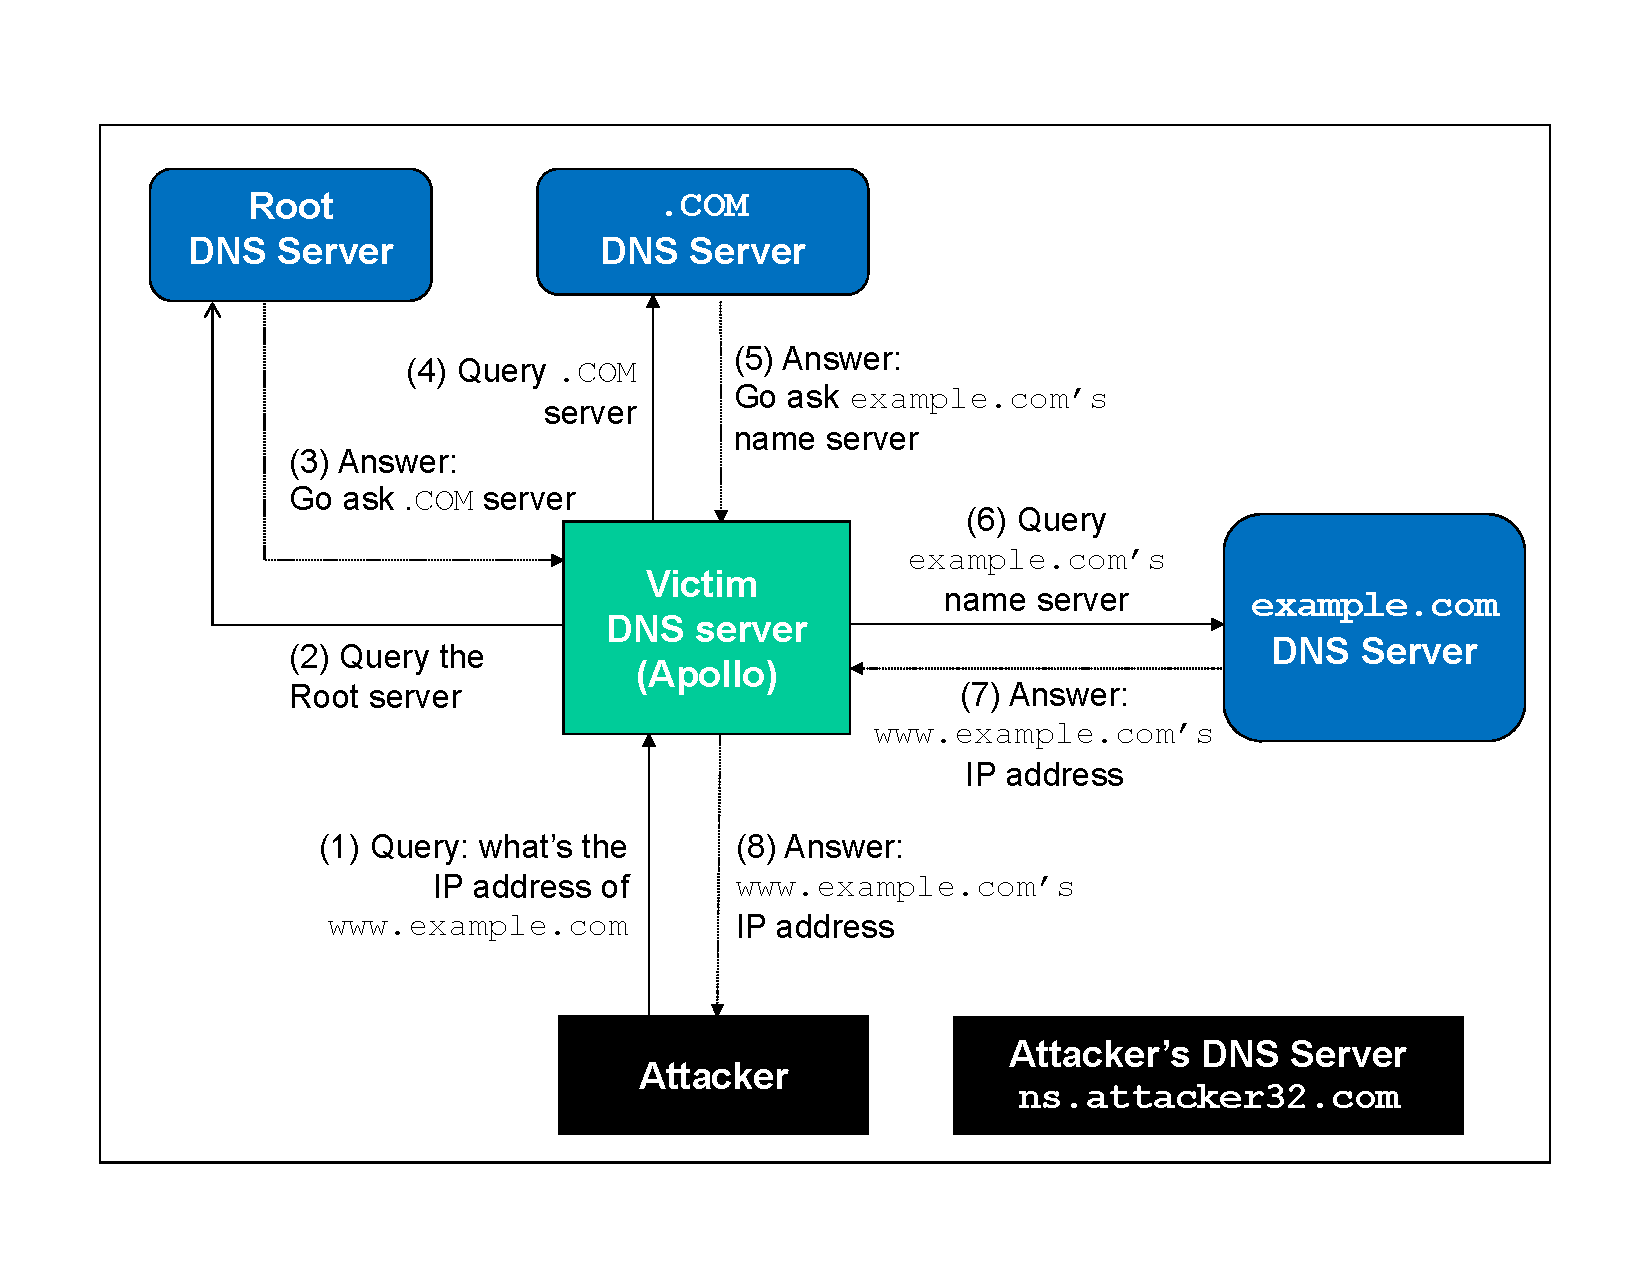
\includegraphics[width=0.9\textwidth]{\dnsFigs/DNS_Remote_new1.pdf}
\caption{El proceso de consulta DNS} 
\label{fig:flow_diagram1}
\end{figure}


\begin{figure}[htb]
\centering
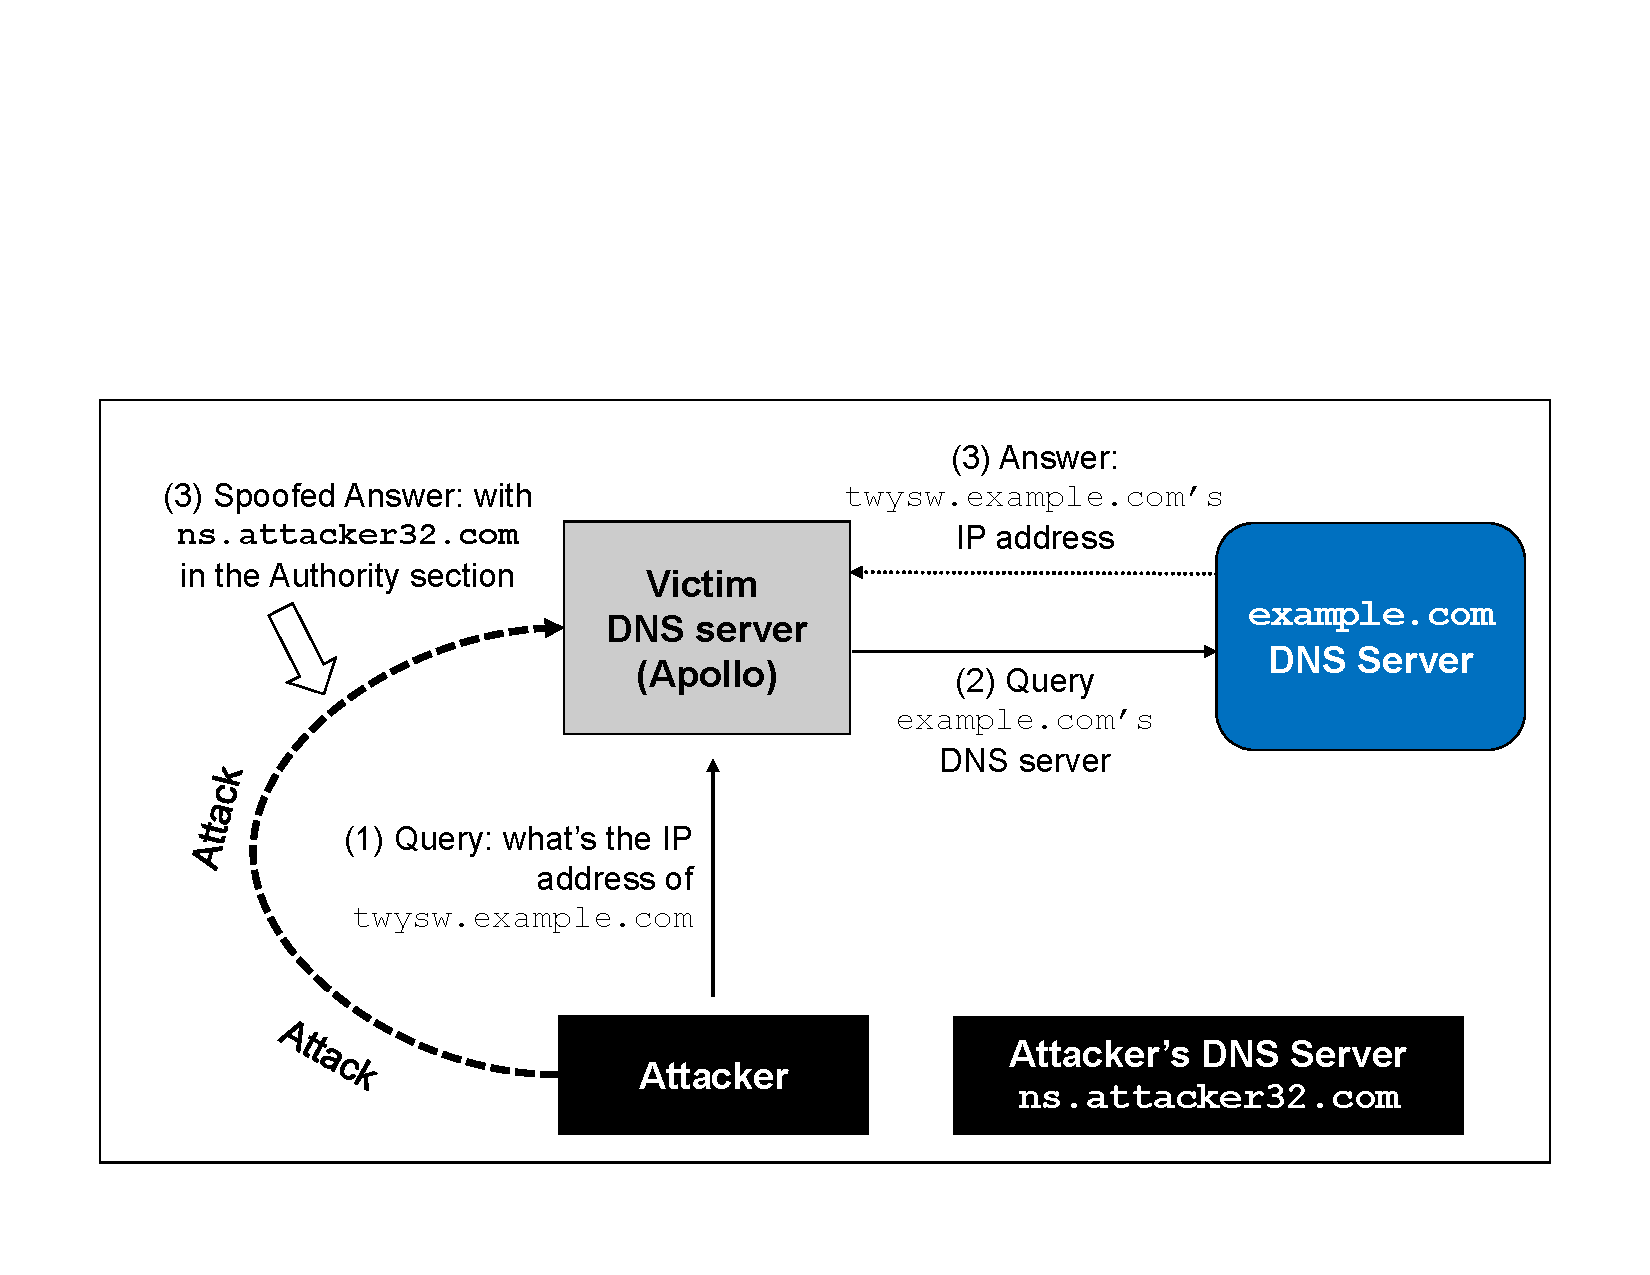
\includegraphics[width=0.9\textwidth]{\dnsFigs/DNS_Remote_new2.pdf}
\caption{El Ataque Kaminsky}
\label{fig:flow_diagram2}
\end{figure}



% -------------------------------------------
% SUBSECTION
% ------------------------------------------- 
\subsection{Como funciona el Ataque de Kaminsky}

En esta tarea, el atacante envía una consulta de petición DNS al servidor DNS de la víctima ({\tt Apollo}), activando una consulta DNS desde {\tt Apollo}.
La consulta puede viajar a través de uno de los servidores DNS raíz, el servidor DNS {\tt .COM} y el resultado final vendrá desde el servidor DNS de {\tt example.com}. Esto se ilustra en la Figura \ref{fig:flow_diagram1}. En caso que la información del nameserver para el dominio {\tt example.com} esté cacheada por {\tt Apollo}, la consulta no irá al servidor raíz o al servidor {\tt .COM}; esto se ilustra en la Figura \ref{fig:flow_diagram2}.
En este laboratorio, la situación representadda en la Figura \ref{fig:flow_diagram2} es la más común, por lo que usaremos esta figura como base para describir el mecanismo de ataque.


While {\tt Apollo} waits for the DNS reply from {\tt example.com}'s name
server, the attacker can send forged replies to {\tt Apollo}, pretending 
that the replies are from {\tt example.com}'s nameserver. If the forged 
replies arrive first, it will be accepted by {\tt Apollo}. The attack will
be successful.


If you have done our local DNS attack lab, you should realize that 
those attacks assume that the attacker and the DNS server are on
the same LAN, i.e., the attacker can observe the DNS query message. 
When the attacker and the DNS server are not on the same LAN,
the cache poisoning attack becomes more difficult.
The difficulty is mainly caused by the fact that the transaction ID
in the DNS response packet must match with that 
in the query packet. Because the transaction ID in the query is 
usually randomly generated, without seeing the query packet,
it is not easy for the attacker to know the correct ID.


Obviously, the attacker can guess the transaction ID. Since the
size of the ID is only 16 bits, if the attacker can forge $K$ 
responses within the attack window (i.e. before the legitimate
response arrives), the probability of success is $K$ over $2^{16}$.
Sending out hundreds of forged responses is not impractical, so
it will not take too many tries before the attacker can succeed. 


However, the above hypothetical attack has overlooked the cache effect.
In reality, if the attacker is not fortunate enough to make a correct guess before
the real response packet arrives, correct information will be cached 
by the DNS server for a while. This caching effect makes it impossible
for the attacker to forge another response regarding the same 
name, because the DNS server will not send out another DNS query for 
this name before the cache times out.
To forge another response on the same name, the attacker has to 
wait for another DNS query on this name, which means he/she has to
wait for the cache to time out. The waiting period can be hours or days.


\paragraph{The Kaminsky Attack.} 
Dan Kaminsky came up with an elegant technique to defeat the caching
effect~\cite{dns:Kaminsky}.
With the Kaminsky attack, attackers will be able to continuously attack
a DNS server on a domain name, without the need for waiting, so
attacks can succeed within a very short period of time.
Details of the attacks are described in~\cite{dns:Kaminsky,seedbook}. 
In this task, we will try this attack method. The following steps with reference to 
Figure~\ref{fig:flow_diagram2} outlines the attack. 

\begin{enumerate}
\item The attacker queries the DNS Server {\tt Apollo} for a non-existing name in 
{\tt example.com}, such as {\tt twysw.example.com},
where {\tt twysw} is a random name. 

\item Since the mapping is unavailable in {\tt Apollo}'s DNS cache, 
{\tt Apollo} sends a DNS query to the nameserver of
the {\tt example.com} domain.

\item While {\tt Apollo} waits for the reply, 
the attacker floods {\tt Apollo} with a stream of spoofed DNS response,
each trying a different transaction ID, hoping one is correct.
In the response, not only does the attacker provide an IP resolution
for {\tt twysw.example.com}, the attacker 
also provides an ``Authoritative Nameservers'' record, indicating 
{\tt ns.attacker32.com} as the nameserver for the {\tt example.com} domain.
If the spoofed response beats the actual responses and
the transaction ID matches with that in the query, 
{\tt Apollo} will accept and cache the spoofed answer, and
and thus {\tt Apollo}'s DNS cache is poisoned.  

\item Even if the spoofed DNS response fails (e.g.
the transaction ID does not match or it comes too late),
it does not matter, because the next time, the attacker will query
a different name, so {\tt Apollo} has to send out another query, 
giving the attack another chance to do the spoofing attack. 
This effectively defeats the caching effect.


\item If the attack succeeds, in {\tt Apollo}'s DNS cache, the
nameserver for {\tt example.com} will be replaced by the attacker's
nameserver {\tt ns.attacker32.com}.
To demonstrate the success of this attack, students need to show that such a record 
is in {\tt Apollo}'s DNS cache. 

\end{enumerate}


\paragraph{Task overview.} Implementing the Kaminsky attack is quite challenging, 
so we break it down into several sub-tasks. 
In Task 2, we construct the DNS request for a random hostname 
in the \texttt{example.com} domain. In Task 3, we construct a spoofed 
DNS reply from \texttt{example.com}'s nameserver.
In Task 4, we put everything together to launch the 
Kaminsky attack. Finally in Task 5, we verify the impact of the attack. 


% -------------------------------------------
% SUBSECTION
% ------------------------------------------- 
\subsection{Tarea 2: Construyendo una petición DNS} 

This task focuses on sending out DNS requests. 
In order to complete the attack, attackers need to trigger the target 
DNS server to send out DNS queries, so they have a chance 
to spoof DNS replies. Since attackers need to try many times before they 
can succeed, it is better to automate the process using a program. 

Students need to write a program to send out DNS queries to the target DNS 
server (i.e., the local DNS server in our setup). 
Students' job is to write this program
and demonstrate (using Wireshark) that their queries can
trigger the target DNS server to send out corresponding DNS queries.
The performance requirement for this task is not high, so
students can use C or Python (using Scapy) to write this code. 
A Python code snippet is provided in the following (the 
\texttt{+++}'s are placeholders; students need to replace them
with actual values): 

\begin{lstlisting}
Qdsec  = DNSQR(qname='www.example.com')
dns    = DNS(id=0xAAAA, qr=0, qdcount=1, ancount=0, nscount=0,
             arcount=0, qd=Qdsec)

ip  = IP(dst='+++', src='+++')
udp = UDP(dport=+++, sport=+++, chksum=0)
request = ip/udp/dns
\end{lstlisting}
 


% -------------------------------------------
% SUBSECTION
% ------------------------------------------- 
\subsection{Tarea 3: Spoofeando respuestas DNS.}   

In this task, we need to spoof DNS replies in the Kaminsky attack. 
Since our target is \texttt{example.com}, we need to spoof
the replies from this domain's nameserver. Students first need to 
find out the IP addresses of \texttt{example.com}'s legitimate 
nameservers (it should be noted that there are multiple 
nameservers for this domain).

Students can use Scapy to implement this task. The following 
code snippet constructs a DNS response packet that includes 
a question section, an answer section, and an NS section. 
In the sample code, we use \texttt{+++} as placeholders; 
students need to replace them with the correct values 
that are needed in the Kaminsky attack. Students need to explain
why they pick those values. 

\begin{lstlisting}
name   = '+++'  
domain = '+++'  
ns     = '+++'

Qdsec  = DNSQR(qname=name)
Anssec = DNSRR(rrname=name,   type='A',  rdata='1.2.3.4', ttl=259200)
NSsec  = DNSRR(rrname=domain, type='NS', rdata=ns, ttl=259200)
dns    = DNS(id=0xAAAA, aa=1, rd=1, qr=1,
             qdcount=1, ancount=1, nscount=1, arcount=0,
             qd=Qdsec, an=Anssec, ns=NSsec)

ip    = IP(dst='+++', src='+++')
udp   = UDP(dport=+++, sport=+++, chksum=0)
reply = ip/udp/dns
\end{lstlisting}
 

Since this reply by itself will not be able to lead to a successful 
attack, to demonstrate this task, students need to 
use Wireshark to capture the spoofed DNS replies, and 
show that the spoofed packets are valid. 


% -------------------------------------------
% SUBSECTION
% ------------------------------------------- 
\subsection{Tarea 4: Ejecutar el Ataque de Kaminsky}   

Now we can put everything together to conduct the Kaminsky attack. 
In the attack, we need to send out many spoofed DNS replies, hoping 
one of them hits the correct transaction number and arrives sooner
than the legitimate replies. Therefore, speed is essential: the more packets 
we can send out, the higher the success rate is. If we use 
Scapy to send the spoofed DNS replies like what we did in the 
previous task, the success rate is too low. Students can use 
C, but constructing DNS packets in C is non-trivial. 
We introduce a hybrid approach using both Scapy and C (see the SEED
book for details). 


With the hybrid approach, we first use Scapy to generate 
a DNS packet template, which is stored in a file. 
We then load this template into a C program, and make 
small changes to some of the fields, and then send 
out the packet. 
We have included a skeleton C code
in \path{Labsetup/Files/attack.c}. 
Students can make changes
in the marked areas. Detailed explanation
of the code is given in the 
guideline section.


\paragraph{Check the DNS cache.}
To check whether the attack is successful or not, we need to 
check the {\tt dump.db} file to see whether our spoofed DNS
response has been successfully accepted by the DNS server. 
The following commands dump the DNS cache, and search whether
the cache contains the word \texttt{attacker} (in our 
attack, we used \texttt{attacker32.com} as the attacker's 
domain; if students use a different domain name, they should 
search for a different word).  

\begin{lstlisting}
# rndc dumpdb -cache && grep attacker /var/cache/bind/dump.db
\end{lstlisting}
 

% -------------------------------------------
% SUBSECTION
% ------------------------------------------- 
\subsection{Task 5: Result Verification}

If the attack is successful, in the local DNS server's DNS cache, 
the {\tt NS} record for \texttt{example.com} will become 
\texttt{ns.attacker32.com}.
When this server receives a DNS query for any hostname
inside the \texttt{example.com} domain,  it will
send a query to \texttt{ns.attacker32.com}, instead of 
sending to the domain's legitimate nameserver. 


To verify whether your attack is successful or not, 
go to the User machine, run the following two
\texttt{dig} commands. In the responses, the IP addresses for 
\texttt{www.example.com} should be the same for both 
commands, and it should be whatever you have included
in the zone file on the Attacker nameserver. 

\begin{lstlisting}
// Ask the local DNS server to do the query
$ dig www.example.com

// Directly query the attacker32 nameserver
$ dig @ns.attacker32.com www.example.com
\end{lstlisting}
 
Please include your observation (screenshots) in the lab 
report, and explain why you think your attack is successful. 
In particular, when you run the first \texttt{dig} commands,
use Wireshark to capture the network traffic, and 
point out what packets are triggered by this
\texttt{dig} command. Use the packet trace to 
prove that your attack is successful. Note that DNS results
may be cached on the local DNS server after the first
\texttt{dig} command is run. This could influence the
results if you run the first \texttt{dig} command before using
Wireshark. You can clear the cache using \texttt{"sudo rndc flush"} 
on the local DNS server, but that will 
require you to redo the attack.



% *******************************************
% SECTION
% ******************************************* 
\section{Guidelines} 

To implement the Kaminsky attack, we can use Scapy to do the packet spoofing. Unfortunately,
the speed of Python is too slow; the number of packets generated per second is too low to
make the attack successful. It is better to use a C program. This could
be quite challenging to many students, because constructing DNS packets using C is not very
easy. I have developed a hybrid method, and have experimented with it in my own class. Using
this approach, students' time spent on coding can be significantly reduced, so they can spend
more time focusing on the actual attack.


The idea is to leverage the strength of both Scapy and C: Scapy is much more convenient in
creating DNS packets than C, but C is much faster. Therefore we simply
use Scapy to create the spoofed DNS packet, and save it to a file.
We then load the packet into a C program. Even though we need to send a 
lot of different DNS packets
during the Kaminsky attack, these packets are mostly the same, except for a few fields. 
Therefore, we can
use the packet generated from Scapy as the basis, find the offsets where
changes need to be made (e.g., the transaction ID field),
and directly make changes. This will be much easier than
creating the entire DNS packets in C.
After the changes are made, we can use the raw socket to send out the packets.
Details of such a hybrid method are provided in
the Packet Sniffing and Spoofing chapter 
of the SEED book~\cite{seedbook}.
The following Scapy program creates a simple DNS reply packet, 
and saves it into a file.


\begin{lstlisting}[caption={\texttt{generate\_dns\_reply.py}}]
#!/usr/bin/env python3
from scapy.all import *

# Construct the DNS header and payload
name   = 'twysw.example.com'
Qdsec  = DNSQR(qname=name)
Anssec = DNSRR(rrname=name, type='A', rdata='1.1.2.2', ttl=259200)
dns    = DNS(id=0xAAAA, aa=1, rd=0, qr=1, 
             qdcount=1, ancount=1, nscount=0, arcount=0, 
             qd=Qdsec, an=Anssec)

# Construct the IP, UDP headers, and the entire packet
ip  = IP(dst='10.0.2.7', src='1.2.3.4', chksum=0)
udp = UDP(dport=33333, sport=53, chksum=0)
pkt = ip/udp/dns

# Save the packet to a file
with open('ip.bin', 'wb') as f:
  f.write(bytes(pkt))
\end{lstlisting}

In a C program, we load the packet from the file \texttt{ip.bin}, and use
it as our packet template, based on which we create many similar packets,
and flood the target local DNS servers with these spoofed replies. For each
reply, we change three places: the transaction ID and the name
\texttt{twysw} occurred in two places (the question section and the answer
section).  The transaction ID is at a fixed place (offset  \texttt{28} from
the beginning of our IP packet), but the offset for the name \texttt{twysw}
depends on the length of the domain name. We can use a binary editor
program, such as \texttt{bless}, to view the binary file \texttt{ip.bin}
and find the two offsets of \texttt{twysw}. In our packet, they are at
offsets \texttt{41} and \texttt{64}.


The following code snippet shows how we make change to these fields. We change
the name in our reply to \texttt{bbbbb.example.com}, and then send out a
spoofed DNS replies, with transaction ID being \texttt{1000}.
In the code, the variable \texttt{ip} points to the beginning of the IP packet.  

\begin{lstlisting}
  // Modify the name in the question field (offset=41)
  memcpy(ip+41, "bbbbb" , 5);

  // Modify the name in the answer field (offset=64)
  memcpy(ip+64, "bbbbb" , 5);

  // Modify the transaction ID field (offset=28)
  unsigned short id = 1000;
  unsigned short id_net_order = htons(id);
  memcpy(ip+28, &id_net_order, 2);
\end{lstlisting}



\paragraph{Generate random names.} In the Kaminsky attack, we need to 
generate random hostnames. There are many ways to do so. The following 
code snippet shows how to generate a random name consisting of 
5 characters. 

\begin{lstlisting}
char a[26]="abcdefghijklmnopqrstuvwxyz";

// Generate a random name of length 5
char name[6];
name[5] = 0;
for (int k=0; k<5; k++)  
   name[k] = a[rand() % 26];
\end{lstlisting}
 



% *******************************************
% SECTION
% ******************************************* 
\section{Informe del Laboratorio}

%%%%%%%%%%%%%%%%%%%%%%%%%%%%%%%%%%%%%%%%

Debe enviar un informe de laboratorio detallado, con capturas de pantalla, para describir lo que ha hecho y lo que ha observado.
También debe proporcionar una explicación a las observaciones que sean interesantes o sorprendentes.
Enumere también los fragmentos de código más importantes seguidos de una explicación. No recibirán créditos aquellos fragmentos de códigos que no sean explicados.
%%%%%%%%%%%%%%%%%%%%%%%%%%%%%%%%%%%%%%%%


% *******************************************
% SECTION
% *******************************************
\section*{Agradecimientos}

Este documento ha sido traducido al Español por Facundo Fontana



%%%%%%%%%%%%%%%%%%%%%%%%%%%%%%%%%%%%%%%%%%
\thispagestyle{empty}
\bibliographystyle{plain}
\def\baselinestretch{1}
\bibliography{BibDNS}
%%%%%%%%%%%%%%%%%%%%%%%%%%%%%%%%%%%%%%%%%%



\end{document}




